\documentclass{article}
\usepackage{amsmath,graphicx,geometry}
\usepackage{xepersian}
%\newcommand{\q}{\newpage\question}
\setlength{\parskip}{3mm}
\setlength{\parindent}{0mm}
\begin{document}
{
\large 
\centering
به نام او

امتحان پایان ترم درس شبکه های مخابراتی

مدت امتحان: 

}

\hrulefill

\Large

سوال 1) درستی یا نادرستی هر یک از گزاره های زیر را با بیان دلایل کافی تعیین کنید.

الف) در پروتکل های دسترسی چندگانه 
\lr{Random Access}
و
\lr{Taking-Turns}
، هنگامی که $M$ نود به طور همزمان از کانالی با نرخ $R$ استفاده می کنند، نرخ ارسال هر یک از نودها مقدار 
$
\frac{R}{M}
$
را خواهد داشت.

ب) در رهیافت \lr{Slotted Aloha} با دو کاربر، اگر احتمال ارسال کاربر A، دو برابر احتمال ارسال کاربر B باشد، نرخ موثر ارسال کاربر A نیز دوبرابر نرخ موثر ارسال کاربر B خواهد بود.

پ) \lr{PGP}
بر مبنای کلیدهای خصوصی و عمومی کار می کند و به کاربر هر دو امکان رمزگذاری (\lr{Encryption}) و امضای دیجیتال (\lr{Digital Signature}) را می دهد.

ت) به کمک 
\lr{nonce}
در \lr{SSL}، می توان از ارسال بسته های تکراری یک کانکشن بسته شده و غیرفعال در یک کانکشن جاری، توسط شخص مزاحم (Intruder) جلوگیری کرد.

(ث) در \lr{Agent Solicitation}، هنگامی که کاربر بیسیمی به شبکه‌ای می پیوندد، \lr{Foreign Agent} آن شبکه سرویس خود را در قالب پیام ICMP شامل آی پی \lr{Agent} و COA به کاربر می‌فرستد.

(ج) \lr{IPsec}، برای کدگذاری دیتاگرام (\lr{datagram}) های لایه‌ی شبکه استفاده می‌شود.

(چ) یکی از موانع پیاده سازی \lr{Collision Detection} در مخابرات بیسیم، مسئله‌ی \lr{Hidden Terminal} است.

\newpage
سوال 2) (امتیازی) در پروتکل \lr{Mobile IP}، فرض کنید کاربری دارای مشخصات زیر است:
\[
\begin{split}
&\text{\lr{Permenant Address = 192.168.1.20}}
\\&\text{\lr{Home Agent Address = 192.168.1.10}}
\end{split}
\]
این کاربر وارد شبکه‌ی جدیدی (\lr{Foreign Network}) با مشخصات زیر می شود:
\[
\begin{split}
&\text{\lr{Foreign Network Subnet Mask = 34.56.112.128/25}}
%\\&\lr{Home Agent Address = 192.168.1.10}
\end{split}
\]

الف) در مرحله \lr{Agent Discovery} با رویکرد \lr{Agent Advertisement}، چگونه آدرس آی پی جدید توسط \lr{Foreign Agent} به این کاربر اختصاص داده می‌شود؟

ب) اگر آدرس آی پی جدید اختصاص داده شده به کاربر (COA)، برابر \lr{34.56.112.153} باشد، چگونه \lr{Home Agent} از این آی پی جدید مطلع می‌شود؟ (مراحل را توضیح دهید.)

پ) هنگامی که کاربر از \lr{Foreign Network} خارج می‌شود، آیا لازم است \lr{Foreign Agent} مربوطه، آدرس آی پی اختصاص داده شده به کاربر (COA) را به طور دستی آزاد کند؟ چرا؟

\newpage
سوال 3) در تکنیک \lr{CSMA/CD}، دو کاربر A و B از یک کانال به طور مشترک استفاده می‌کنند. هر کاربر پس از آشکارسازی $n$ تصادم برای هر بسته خود، به اندازه $K$ تا ارسال بعدی بسته صبر می‌کند که $K$ به تصادف از بازه‌ی 
$
\{0,1,2,\cdots ,2^n-1\}
$
(بر حسب میلی ثانیه) انتخاب شده است. فرض کنید ارسال هر بسته، دقیقا 1 میلی ثانیه طول می‌کشد و هر دو کاربر با شروع از تایم ابتدای تایم اسلات اول، بسته های خود را به طور پشت سر هم می‌فرستند.

الف) با چه احتمالی، کاربر A بسته‌ی اول خود را در تایم اسلات سوم با موفقیت ارسال می‌کند؟

ب) اگر در یک تایم اسلات خاص، کاربر های A و B، به ترتیب $m$ و $n$ تصادم را برای بسته خود تجربه کنند، با چه احتمالی در دو تایم اسلات بعدی تصادمی \underline{رخ نمی‌دهد}؟

\newpage
سوال 4) در شبکه‌ی زیر که دو زیرشبکه (subnet) توسط یک روتر به هم متصل شده اند:
\begin{figure}[htbp]
\centering
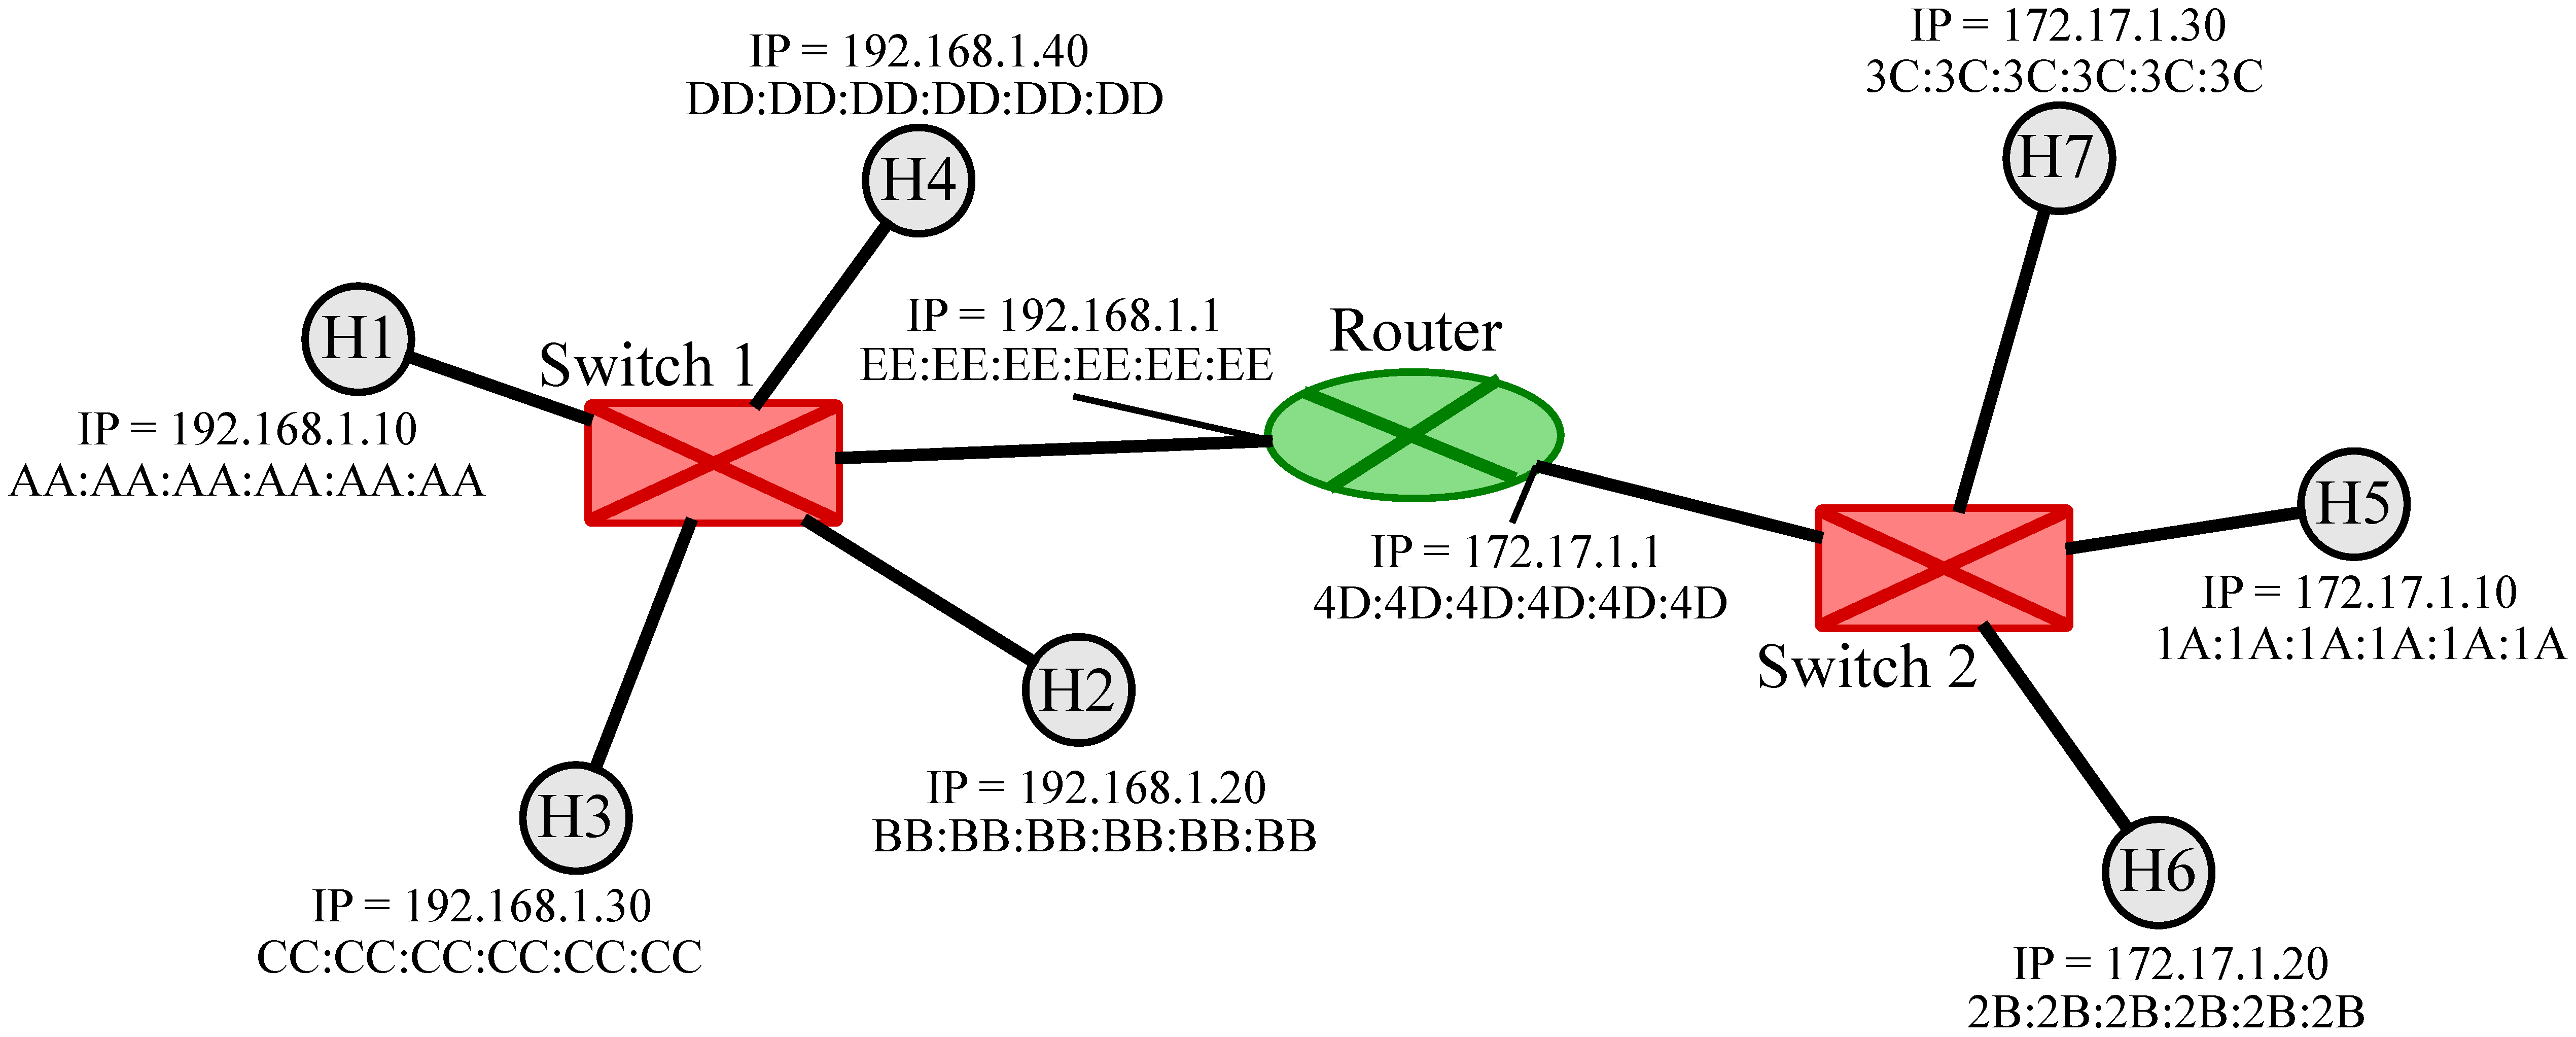
\includegraphics[width=150mm]{link_layer_1.eps}
\end{figure}

الف) اگر \lr{H1} بخواهد پیامی را به \lr{H2} بفرستد و \lr{Lookup Table} سوئیچ ها خالی باشد، این پیام به کدام یک از نودهای 
\lr{H2}
تا 
\lr{H7}
فوروارد می‌شود؟ چرا؟

ب) اگر \lr{H1} بخواهد پیامی را به \lr{H5} بفرستد، با فرض آن که \lr{ARP table} در تمام نودها و همچنین \lr{Lookup Table} سوئیچ کامل باشد، مک آدرس و آی پی آدرس مبدا و مقصد را در \lr{frame} هایی که از سوئیچ 1 به پورت \lr{P1} روتر و از پورت \lr{P2} روتر به سوئیچ 2 می روند را بنویسید.

پ) فرض کنید بخواهیم دو \lr{subnet} مستقل ایجاد کنیم که \lr{subnet} اول شامل نودهای 
\lr{H1}
و
\lr{H2}
و \lr{subnet} دیگر شامل نودهای 
\lr{H3}
و
\lr{H4}
باشد. بدین منظور، برای دستکاری تنظیمات سوئیچ 1 چه تکنیکی را پیشنهاد می‌کنید؟ توضیح دهید چگونه این تکنیک، نیاز شما را برآورده می‌کند.

\newpage
سوال 5) در مراحل رمزگذاری زیر، فرض کنید بلوک دایره الحاق دو رشته به هم را نشان می‌دهد. آلیس میخواهد پیام m را رمزگذاری کرده و به باب منتقل کند. فرض کنید کلید های خصوصی و عمومی آلیس به ترتیب
$
K_A^-
$
و
$
K_A^+
$
و کلیدهای خصوصی و عمومی باب به ترتیب
$
K_B^-
$
و
$
K_B^+
$
باشند.
\begin{figure}[htbp]
\centering
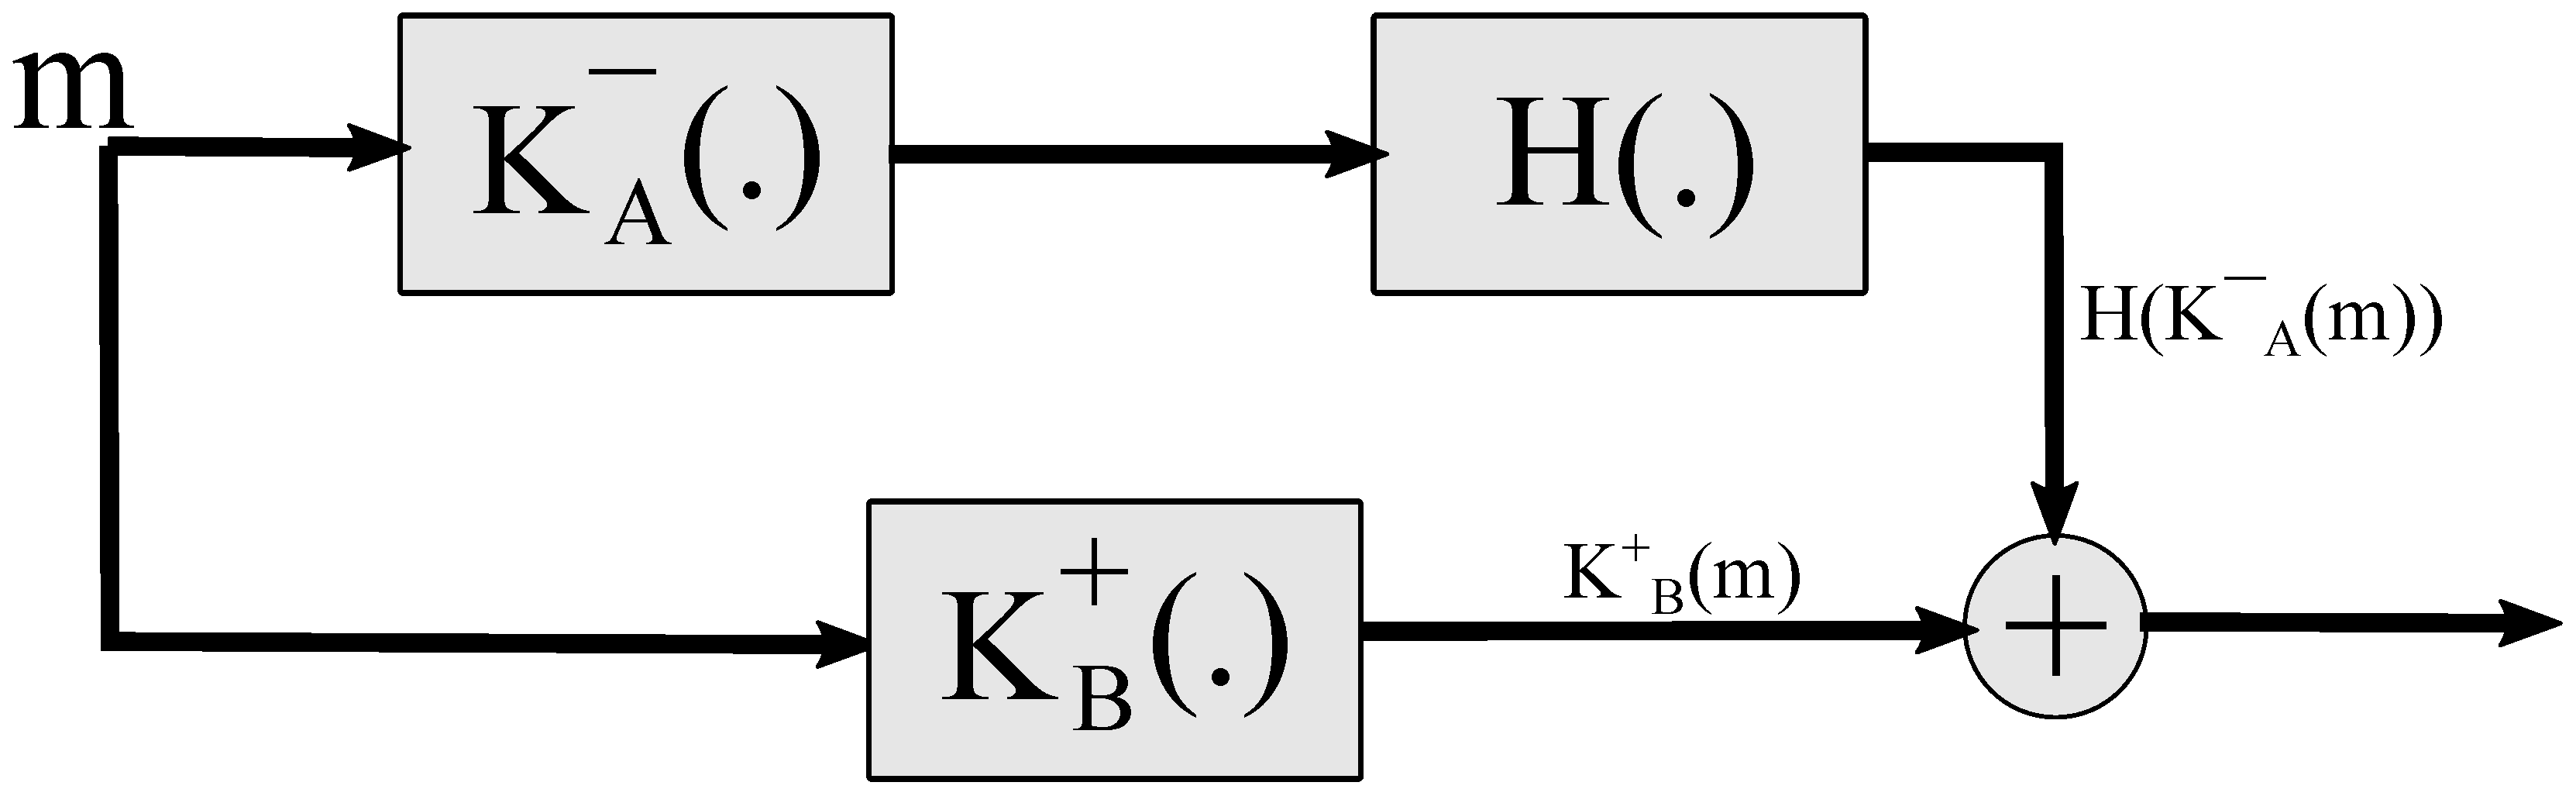
\includegraphics[width=100mm]{crypto.eps}
\end{figure}

الف) آیا تمام موارد محرمانگی پیام (Confidentiality)، اصالت پیام (Authentication) و تمامیت پیام (\lr{Message Integrity}) حفظ شده اند؟ هر مورد را توضیح دهید.

ب) باب در هنگام رمز گشایی پیام و تایید هویت فرستنده (Authentication) به چه مشکلی بر می‌خورد؟ راه حل این مشکل چیست؟

پ) پس از رفع مشکل قسمت ب، بلوک دیاگرام لازم را برای رمزگشایی پیام رسم کنید.

\newpage
سوال 6) برای \lr{firewall} یک شبکه داخلی، جدولی زیر را به گونه ای تکمیل کنید که
\begin{itemize}
\item
به کاربران داخلی شبکه، اجازه‌ی ارسال پکت به کاربران خارج شبکه را روی تمام پورت ها بدهد.
\item
به کاربران داخلی شبکه، اجازه‌ی ارتباط با سروری با آی پی \lr{172.17.15.234} خارج از شبکه را روی پورت های 0 تا 1023 بدهد.
\item
جلوی ارسال بسته از شبکه ای با 
\lr{subnet mask = 10.33.12.16/28}
را بگیرد.
\end{itemize}
\begin{figure}[htbp]
\centering
\includegraphics[width=100mm]{firewall.png}
\end{figure}












\end{document}